% Unofficial Butler University LaTeX
% https://github.com/andiac/gemini-cam
% a fork of https://github.com/anishathalye/gemini
% also refer to https://github.com/k4rtik/uchicago-poster
% and https://github.com/andiac/gemini-cam


\documentclass[final]{beamer}

% ====================
% Packages
% ====================

\usepackage[T1]{fontenc}
\usepackage{lmodern}
\usepackage[size=custom,width=91.44,height=60.96,scale=0.80]{beamerposter}
%size is scaled to 36in x 24in (in cm). Use "scale=##" parameter to enlarge or reduce font size to fit as needed, depending on total word count.
\usetheme{gemini}
\usecolortheme{bulldog}
\usepackage{graphicx}
\usepackage{booktabs}
\usepackage{tikz}
\usepackage{pgfplots}
\pgfplotsset{compat=1.14}
\usepackage{anyfontsize}
\renewcommand{\arraystretch}{1.2}

% ====================
% Lengths
% ====================

% If you have N columns, choose \sepwidth and \colwidth such that
% (N+1)*\sepwidth + N*\colwidth = \paperwidth
\newlength{\sepwidth}
\newlength{\largecolwidth}
\newlength{\smallcolwidth}
\setlength{\sepwidth}{0.025\paperwidth}
\setlength{\largecolwidth}{0.4\paperwidth}
\setlength{\smallcolwidth}{0.25\paperwidth}

\newcommand{\separatorcolumn}{\begin{column}{\sepwidth}\end{column}}

% ====================
% Title
% ====================

\title{Monitoring Hate Speech and Offensive Language on Social Media}

\author{Sidney Gig-Jan Wong \inst{1}\inst{2}}

\institute[shortinst]{\inst{1} Geospatial Research Institute\samelineand \inst{2} University of Canterbury}

% ====================
% Footer (optional)
% ====================

\footercontent{
  \href{https://geospatial.ac.nz/}{https://geospatial.ac.nz/} \hfill
  Fourth Spatial Data Science Symposium 2023 \hfill
  \href{mailto:sidney.wong@pg.canterbury.ac.nz}{sidney.wong@pg.canterbury.ac.nz}}
% (can be left out to remove footer)

% ====================
% Body
% ====================

\begin{document}

% Refer to https://github.com/k4rtik/uchicago-poster
% logo: https://www.cam.ac.uk/brand-resources/about-the-logo/logo-downloads
\addtobeamertemplate{headline}{}
{
    \begin{tikzpicture}[remember picture,overlay]
      \node [anchor=north west, inner sep=2.5cm] at ([xshift=0.0cm,yshift=1.0cm]current page.north west)
      {
\includegraphics[height=4.5cm]{figures/gri.png}}; 
    \end{tikzpicture}

    \begin{tikzpicture}[remember picture,overlay]
      \node [anchor=north east, inner sep=2.5cm] at ([xshift=0.0cm,yshift=1.0cm]current page.north east)
      {
\includegraphics[height=4.5cm]{figures/uc.png}}; 
    \end{tikzpicture}
}

\begin{frame}[t]
\begin{columns}[t]
\separatorcolumn

\begin{column}{\smallcolwidth}

    \begin{alertblock}{Content Warning}
  
   This poster contains references to and descriptions of hate speech and offensive language.

   \end{alertblock}
  
  \begin{block}{Background}
    
    Hate speech and offensive language content on social media platforms has increased in both volume and tone since early-2023 \cite{hattotuwa_transgressive_2023}. These insights were largely based on qualitative accounts. The main contribution of this study is to offer an innovative method to monitor levels of hate speech and offensive language content on social media across Aotearoa New Zealand.

  \end{block}
  
  \begin{block}{Methodology}

    We used georeferenced Twitter data from the Corpus of Global Language Use \cite{dunn_mapping_2020}. The georeferenced tweets originated from within a 50-kilometre radius for each of the 100 data collection points across Aotearoa as shown in Figure \ref{fig:1}. Data collection has been on-going since June 2018. 
  
    \begin{figure}
        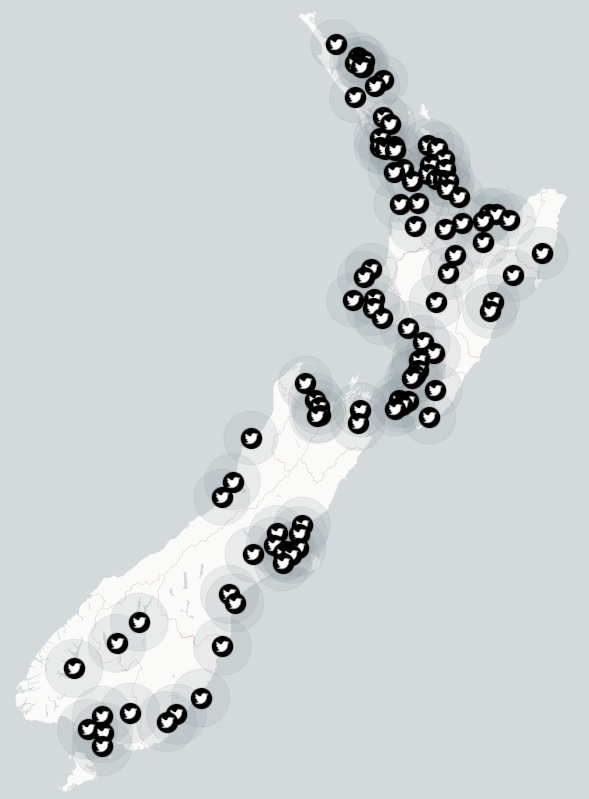
\includegraphics[width=0.4\textwidth]{figures/map_aotearoa.png}
        \caption{Map of data collection points across Aotearoa}
        \label{fig:1}
    \end{figure}

    We pretrained XLM-RoBERTa \cite{conneau_unsupervised_2020} with 50,000 samples of tweets from Aotearoa to fine-tune the language embeddings. We then trained a text multi-class text classification model using an open source hate speech data set \cite{davidson_automated_2017}. Our final classification model had an average weighted F1 score of 0.90. An overview of our system is shown in Figure \ref{fig:2}.
    \\~\
  \usetikzlibrary{arrows.meta,chains,
    positioning,shapes.geometric}

    \begin{figure}
    \centering
    \begin{tikzpicture}[
        node distance = 5mm and 7mm,
        start chain = going right,
        disc/.style = {
            shape=cylinder,
            draw,
            shape aspect=0.3,
            shape border rotate=90,
            text width=25mm, 
            align=center, 
            font=\tiny\linespread{0.8}\selectfont},
        mdl/.style = {
            shape=ellipse, 
            draw,
            align=center,
            text width=25mm,
            font=\tiny\linespread{0.8}\selectfont},
        alg/.style = {
            draw, 
            align=center,
            text width=25mm,
            font=\tiny\linespread{0.8}\selectfont}]
        \begin{scope}[every node/.append style={on chain, join=by -Stealth}]
            \node (n1) [mdl] {Pretrained Language Model};
            \node (n2) [alg] {Language\\ Modelling};
            \node (n3) [mdl] {Retrained Language Model};
            \node (n4) [alg] {Text\\ Classification};
            \node (n5) [mdl] {Classification Language Model};
        \end{scope}
            \node (s6) [below=of n2]  {Step 1: Pretraining};
            \node (s7) [below=of n4]  {Step 2: Finetuning};
            \node (s8) [above=of n1] [disc] {Training\\ data};
            \node (s9) [above=of n3] [disc] {Training\\ data};
        % arrows
        \draw[->] (s8) -- (n1);
        \draw[->] (s9) -- (n3);
    
    \end{tikzpicture}

    \caption{System Overview}
    \label{fig:2}
    
    \end{figure}

    We applied our text classification system on a random monthly sample of 1,000 tweets per location with replacement.
    \end{block}

\end{column}

\separatorcolumn

\begin{column}{\largecolwidth}

  \begin{exampleblock}{Key Findings}

    We took a transformer-based language approach using pretrained language models (PLMs) to develop a hate speech/offensive language classification system. We found that:

    \begin{itemize}
        \item Language models are a useful tool in monitoring social media behaviour
        \item Open source hate speech data sets may not be relevant within the context of Aotearoa
    \end{itemize}

    Therefore, we suggest further work is needed to develop language training data specific to the social, political, and linguistic context of Aotearoa.
  
  \end{exampleblock} 
  
  \begin{block}{Results}

  We ran the text classification model on the monthly samples of tweets for each location. The combined national totals for Aotearoa are presented in Table \ref{tab:1}. We calculated the proportion (\%) of tweets predicted as the sum of hate speech or offensive language for each location. The results show that the occurrence of hate speech and offensive language based on the classification model were increasing between the annual periods 2018-2019 to 2021-2022.
  \\~\
  
    \begin{table}
    \small
    \centering
    \begin{tabular}{lccc}
    \hline
    \textbf{Year} & \textbf{Hate Speech (n)} & \textbf{Offensive Language (n)} & \textbf{Proportion (\%)} \\
    \hline
    2018-2019 & 540 & 29,373 & 4.35\\
    2019-2020 & 581 & 33,279 & 4.52\\
    2020-2021 & 577 & 34,398 & 4.53\\
    2021-2022 & 588 & 30,563 & 4.23\\
    2022-2023 & 486 & 27,569 & 4.28\\
    \hline
    \end{tabular}
    \caption{\label{tab:1} The occurrence of hate speech and offensive language for each period starting June 1 and ending May 31 the following year in Aotearoa.}
    \end{table}

  Figure \ref{fig:3} plots the proportion of hate speech and offensive language by month. We compared the local measures for individual locations, the regional mean, and the national mean. Due to the paucity of results for some locations, we combined some of the regional council areas in Figure \ref{fig:3} as some locations were unable to yield monthly samples of 1,000 tweets. The West Coast/Otago/Southland area exhibited the highest proportion of hate speech and offensive language based on the classification model.
 
    \begin{figure}
        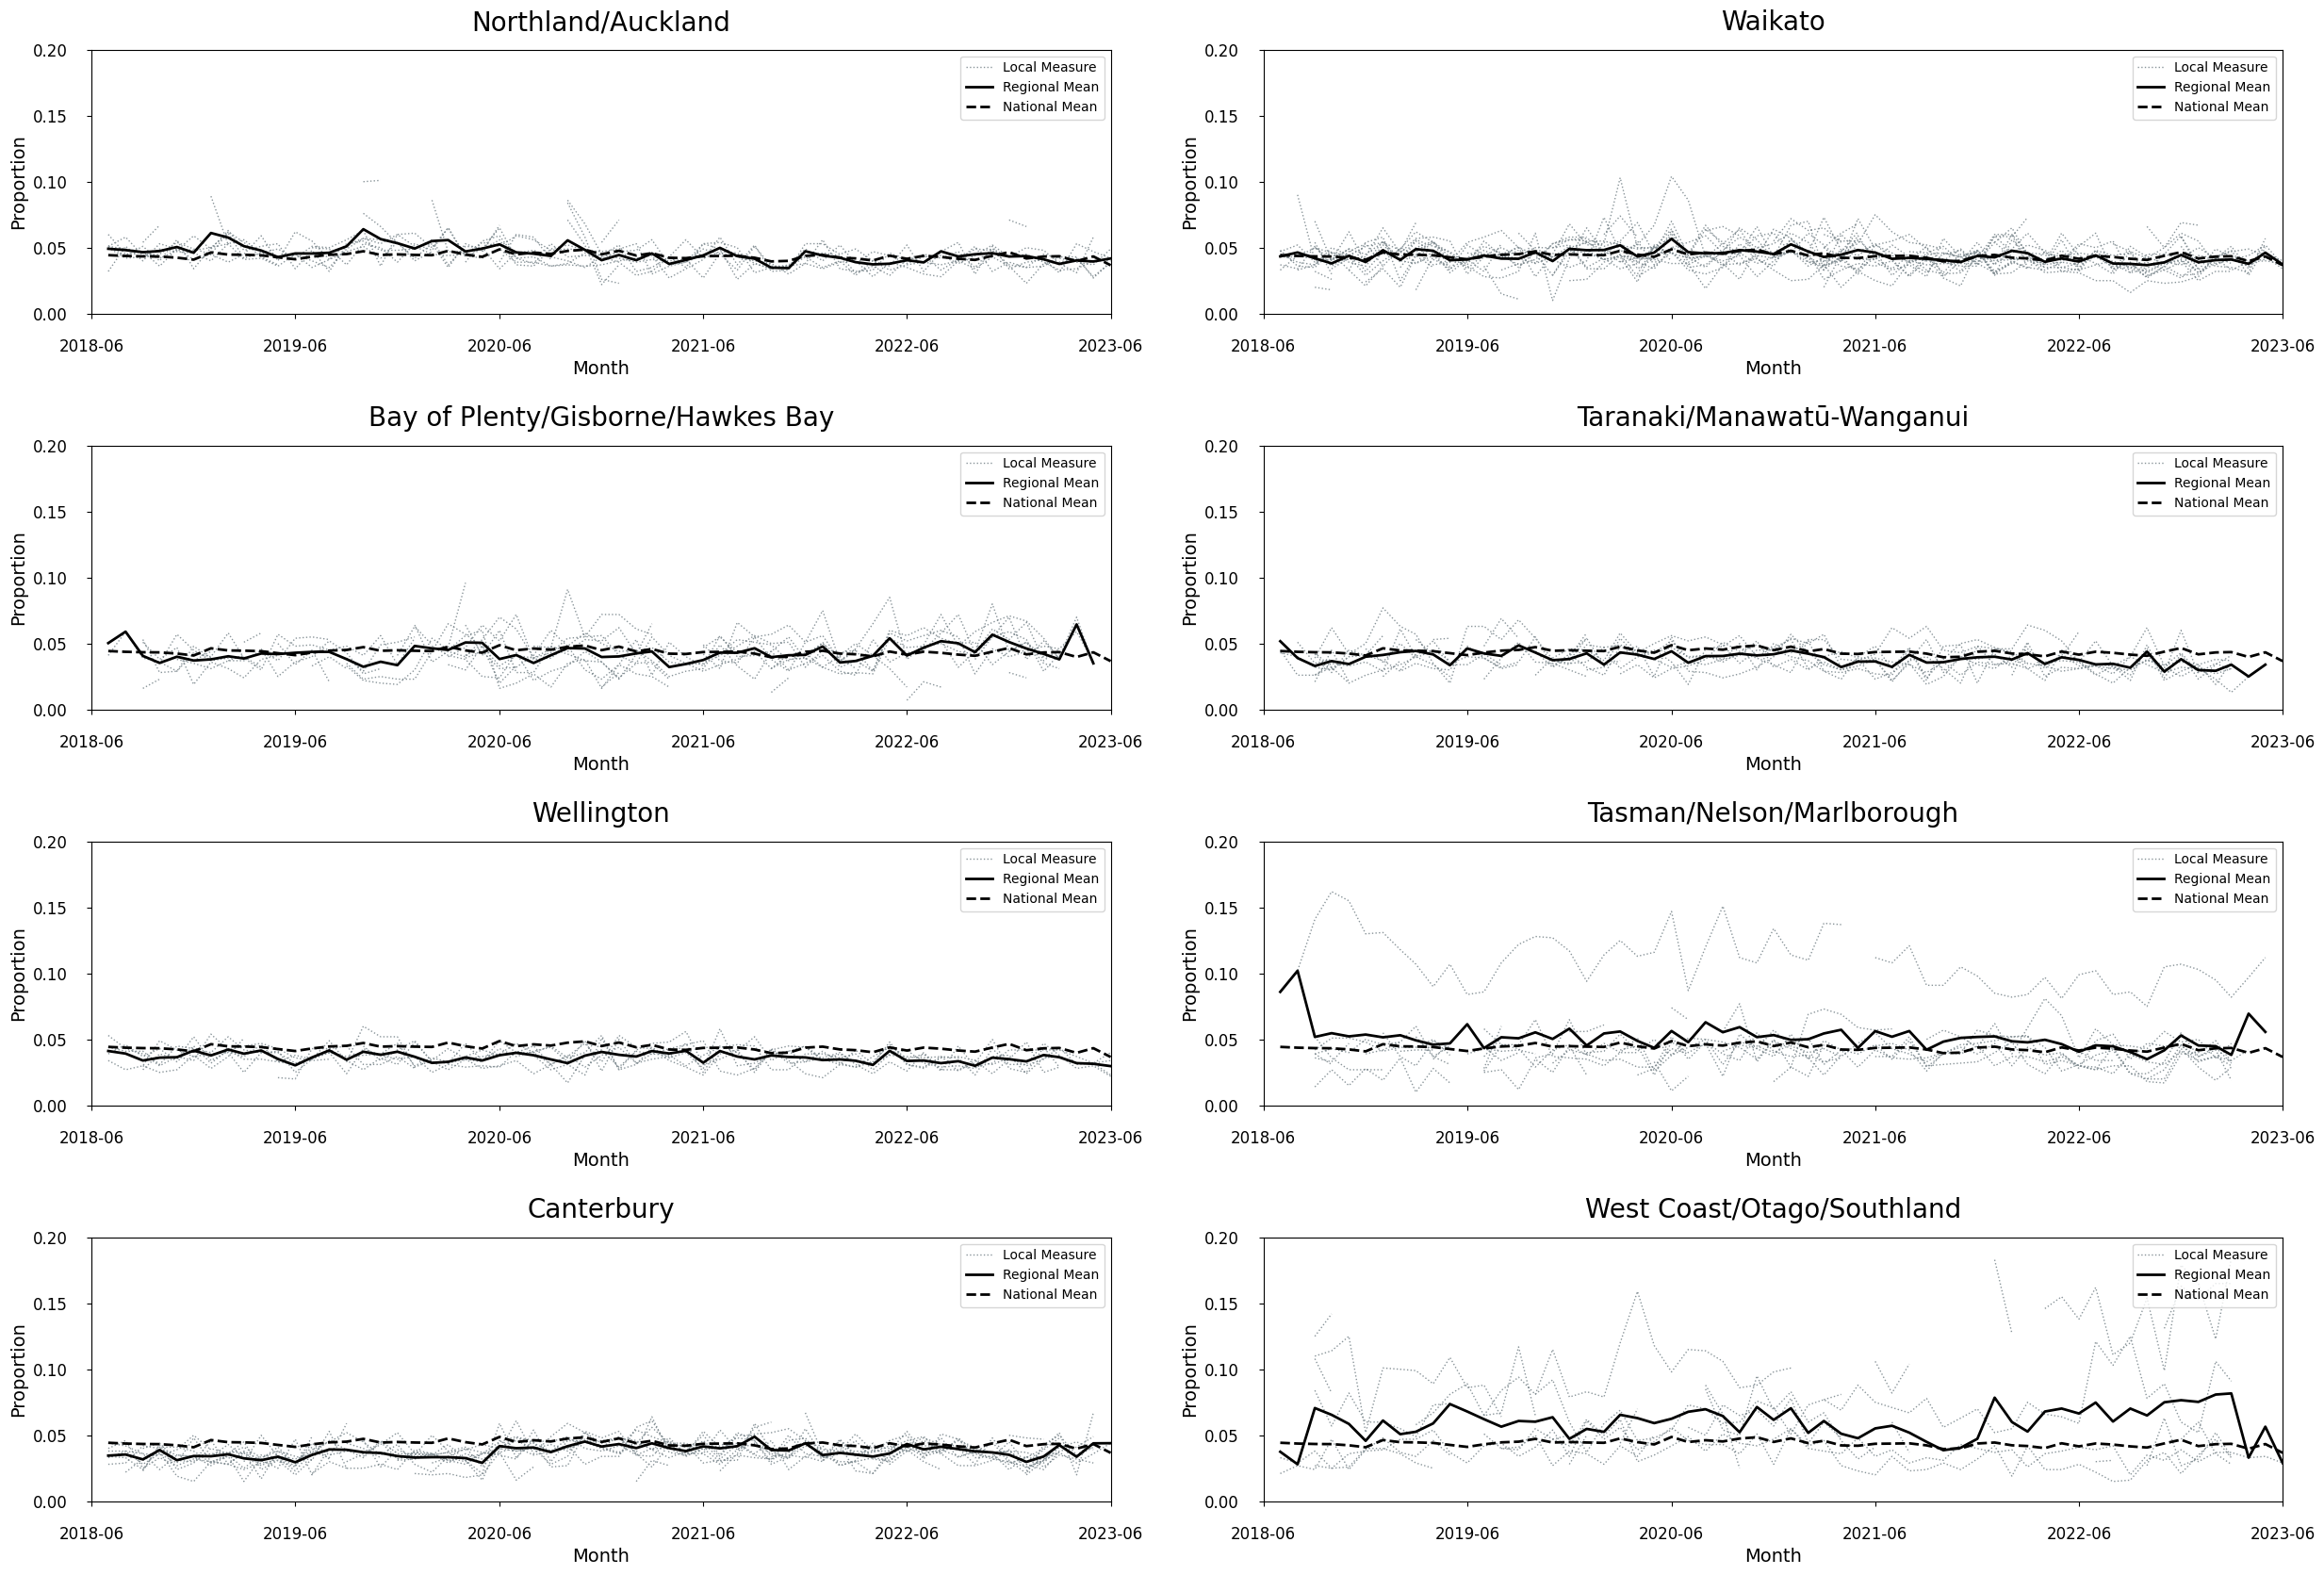
\includegraphics[width=0.8\textwidth]{figures/figure_proportions.png}
        \caption{Proportion of hate speech and offensive tweets by broad regional areas}
        \label{fig:3}
    \end{figure}

  \end{block}

\end{column}

\separatorcolumn

\begin{column}{\smallcolwidth}

  \begin{block}{Discussion}

  The results suggest that the occurrence of hate speech and offensive language on social media has increased across Aotearoa. The results also suggest:
  
  \begin{itemize}
      \item Urban areas had similar rates of hate speech and offensive language when compared with the national mean
      \item Rural areas had higher rates of hate speech and offensive language when compared with the national mean
  \end{itemize}

  A closer inspection of the predicted tweets found that many of the samples would not be considered hate speech in the Aotearoa as shown in the word cloud in Figure \ref{fig:4} with stop words removed and slurs censored.
  
  \begin{figure}
    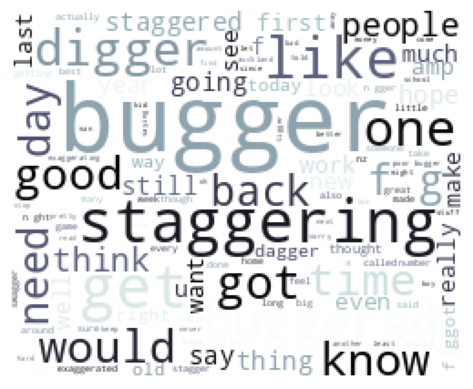
\includegraphics[width=0.6\textwidth]{figures/word_cloud.png}
        \caption{Word cloud of hate speech predicted by the classification model}
        \label{fig:4}    
    \end{figure}

    \end{block}

    The hate speech data set produced by  used to train the classification model was not designed based on the social, political, or linguistic context of Aotearoa \cite{davidson_automated_2017}. What might be a dialect feature words which  (e.g., 'bugger') could be considered hate speech or offensive language outside the Aotearoa context. Furthermore, words which may contain structural similarities with slurs will be erroneously misclassified.
    
    \begin{block}{Conclusion}

    Despite the usefulness of language models to monitor social media behaviour such as hate speech and offensive language, we need to ensure that the language training data is relevant to a particular social, political, or linguistic context. We propose further work is needed to develop hate speech training data specific to Aotearoa.
    
  \end{block}

  \begin{block}{References}

    \nocite{*}
    \footnotesize{\bibliographystyle{plain}\bibliography{references}}

  \end{block}

\end{column}

\separatorcolumn
\end{columns}
\end{frame}

\end{document}
